\section{AiM}

\paragraph{}
Another company that makes data loggers to attach to a vehicle is AiM Sports \cite{AiMSite}.
AiM makes data loggers that are specifically intended for motorsport applications as well as other products such as dashboards, steering wheels, and ECUs.
Similarly to AEM, AiM also makes combined dashes and loggers, as well as different accessories and sensors for their dashboards and loggers.

\subsection{AiM Loggers}

\paragraph{}
AiM develops several loggers with similar specs to the AEM loggers with some additional features.
One such logger, the MXS 1.3 is shown in \cref{fig:AIM_TFT}.
The MX series and MXM series loggers are comparable to the CD5 and CD7 logger dashes that are sold by AEM.
These loggers also act as dash displays, with the MX series having a nicer display than the MXM series.
The MX series and the MXM series both support many different ECU communication protocols over CAN or RS-232 as well as several different direct sensor inputs.

\begin{figure}[H]
	\centering
	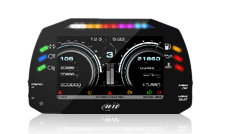
\includegraphics[width=\linewidth]{AIM_TFT_DASH.png}
	\caption{AIM MXS 1.3 Dashboard}
	\label{fig:AIM_TFT}
\end{figure}

\paragraph{}
AiM also develops loggers that do not serve as a dash, only containing the functionality for aggregating and logging data.
These loggers offer most of the same features that the dash loggers offer, with CAN connectivity, wireless connectivity, and different direct sensor inputs.
There are two main products offered in this line, the ECULog and the XLog.
The ECULog is the cheaper version with fewer features, only supporting external sensor inputs and communication.
The XLog includes all of this and an onboard IMU and GPS, making it easier to monitor vehicle position and behavior during a lap.

\subsection{AiM Add-Ons}

\paragraph{}
To communicate with sensors, there are a few required accessories needed.
These are a data hub that can be used to communicate with different accessories and a channel expansion to provide more ports for connecting different sensors to the CAN network.
The channel expansion ports provide power and ground signals, as well as an analog sensor input for reading the sensor data.
The data hub just acts as a way to reduce the number of devices directly connected to the logger itself.
These devices cannot be purchased directly from AiM and instead must be purchased from a retailer like Summit.
On Summit's website, the data hub is \$77, and the channel expansions are \$288, making them somewhat expensive requirements for using sensors.

\paragraph{}
Besides these essential add-ons, there are some other useful add-ons.
AiM makes a GPS add-on shown in \cref{fig:AIM_GPS} that can provide location data, as well as a thermocouple hub that can be used similarly to the thermocouple add-on that AEM makes.
They also make a storage expansion option, to increase the total amount of data that can be stored on board.
None of these add-ons are required to utilize the system and to log data, but they are useful tools that improve the system and provide some useful functionality.

\begin{figure}[H]
	\centering
	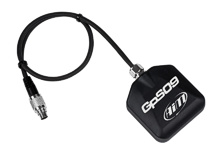
\includegraphics[width=\linewidth]{AIM_GPS.jpg}
	\caption{AiM GPS09C GPS Module}
	\label{fig:AIM_GPS}
\end{figure}

\paragraph{}
In addition to the hardware accessories to improve the experience and connectivity of AiM data loggers, AiM also sells different kinds of sensors for automotive applications.
These include temperature sensors, pressure sensors, combined temperature and pressure sensors, position sensors, speed sensors, and rpm sensors.
Most of these sensors have analog voltage outputs, meaning that to communicate with the data logger, these sensors must be connected to the logger directly or to a unit that can transmit the data over CAN or other supported communication protocols.
These sensors, like the other add-ons and loggers, cannot be purchased directly from AiM and must be purchased from a third-party retailer.
The pricing on sensors is similar to the pricing of similar sensors sold by AEM.

\paragraph{}
AiM utilizes a tool called CAN builder to set up the logger to properly handle and process CAN inputs.
This tool is essentially a graphical interface for configuring the logger to properly read CAN messages.
CAN builder is capable of interfacing with AiM's proprietary XC1 file types, the standard DBC file types, or building a custom driver for reading CAN messages.
The CAN builder tool can only be used on AiM devices that are supported by their Race Studio 3 software.